% Chapter 4: Numerical Computation

\chapter{Numerical Computation}
\label{chap:numerical-computation}

This chapter covers numerical methods and computational considerations essential for implementing deep learning algorithms. Topics include gradient-based optimization, numerical stability, and conditioning.

\begin{learningobjectives}
\objective{Numerical precision issues and recognize how finite precision arithmetic affects deep learning computations and implement solutions for overflow, underflow, and numerical instability}
\objective{Gradient-based optimization and apply gradient descent and understand the role of Jacobian and Hessian matrices in optimization landscapes, including critical points and saddle points}
\objective{Constrained optimization and use Lagrange multipliers and KKT conditions to solve optimization problems with constraints, relevant for regularization and fairness in deep learning}
\objective{Numerical stability and calculate condition numbers, identify ill-conditioned problems, and implement gradient checking and other numerical verification techniques}
\objective{Practical numerical techniques and use log-sum-exp tricks, mixed precision training, and other numerical stability methods in real deep learning implementations}
\objective{Numerical issues and recognize common numerical problems in deep learning and apply appropriate solutions for robust model training}
\end{learningobjectives}

% Chapter 4, Section 1: Overflow and Underflow

\section{Overflow and Underflow \difficultyInline{beginner}}
\label{sec:overflow-underflow}

Overflow and underflow are critical numerical issues that occur when computations produce values outside the representable range of floating-point arithmetic, causing catastrophic failures in deep learning algorithms that rely on precise numerical calculations.

\subsection{Intuition: The Problem with Finite Precision}

Imagine you're trying to measure the height of a building using a ruler that only has markings every meter. If the building is 10.7 meters tall, you might record it as 11 meters - you've lost some precision. Now imagine doing millions of calculations with this imprecise ruler, and you can see how small errors can compound into big problems. Computers face a similar challenge because they can only represent a finite number of digits, so they must round numbers, which is like having a ruler with limited markings where some information is always lost. In deep learning, this becomes critical because neural networks perform millions of calculations where small errors accumulate, exponential functions are common and can produce extremely large or small numbers, and gradients can become very small and might round to zero, breaking training. Computers represent real numbers with finite precision, typically using floating-point arithmetic, which leads to rounding errors that can accumulate and cause problems in deep learning algorithms.

\subsection{Floating-Point Representation}

The IEEE 754 standard defines floating-point numbers using a fixed number of bits to represent real numbers, with 32-bit floats having a smallest positive number of approximately $10^{-38}$, a largest number of approximately $10^{38}$, and a machine epsilon of approximately $10^{-7}$. This representation allows computers to handle a wide range of numbers but introduces limitations that can cause overflow when numbers exceed the maximum representable value and underflow when numbers become smaller than the minimum representable value.

\begin{figure}[h]
\centering
\begin{tikzpicture}
\begin{axis}[
    ylabel={Representable Numbers},
    xlabel={Value (log scale)},
    xmode=log,
    ymin=0,
    ymax=1,
    width=12cm,
    height=6cm,
    xtick={1e-40, 1e-30, 1e-20, 1e-10, 1, 1e10, 1e20, 1e30, 1e40},
    xticklabels={$10^{-40}$, $10^{-30}$, $10^{-20}$, $10^{-10}$, $1$, $10^{10}$, $10^{20}$, $10^{30}$, $10^{40}$},
    ytick=\empty
]
% Underflow region
\addplot[bookred, thick, domain=1e-50:1e-38] {0.2};
\node[bookred] at (axis cs: 1e-45, 0.3) {Underflow};

% Normal range
\addplot[bookpurple, thick, domain=1e-38:1e38] {0.5};
\node[bookpurple] at (axis cs: 1, 0.6) {Normal Range};

% Overflow region
\addplot[bookred, thick, domain=1e38:1e50] {0.8};
\node[bookred] at (axis cs: 1e45, 0.9) {Overflow};
\end{axis}
\end{tikzpicture}
\caption{Representable range for 32-bit floating-point numbers}
\label{fig:float-range}
\end{figure}

\subsection{Underflow}

\subsubsection{Intuition: When Numbers Become Too Small}

Think of underflow like trying to measure the width of a human hair with a ruler marked in meters. The hair is so thin that your ruler shows 0 meters - you've lost all information about the actual size.

In computers, \textbf{underflow} occurs when numbers become so small that they round to zero. This is like your ruler being too coarse to measure tiny objects.

\textbf{Underflow} occurs when numbers near zero are rounded to zero. This can be problematic when we need to compute ratios or logarithms. For example, the softmax function:

\begin{equation}
\text{softmax}(\vect{x})_i = \frac{\exp(x_i)}{\sum_j \exp(x_j)}
\end{equation}

can underflow if all $x_i$ are very negative.

\subsection{Overflow}

\subsubsection{Intuition: When Numbers Become Too Large}

Imagine trying to count the number of atoms in the universe using a calculator that can only display 8 digits. When you reach 99,999,999, the next number would be 100,000,000, but your calculator shows "Error" or resets to 0.

\textbf{Overflow} occurs when large numbers exceed representable values. In the softmax example, overflow can occur if some $x_i$ are very large.

\subsection{Numerical Stability}

To stabilize softmax, we use the identity:

\begin{equation}
\text{softmax}(\vect{x}) = \text{softmax}(\vect{x} - c)
\end{equation}

where $c = \max_i x_i$. This prevents both overflow and underflow.

Similarly, when computing $\log(\sum_i \exp(x_i))$, we use the \textbf{log-sum-exp} trick:

\begin{equation}
\log\left(\sum_i \exp(x_i)\right) = c + \log\left(\sum_i \exp(x_i - c)\right)
\end{equation}

\subsubsection{Example: Softmax Numerical Issues}

Consider computing softmax for $\vect{x} = [1000, 1001, 1002]$:

\textbf{Naive approach:}
\begin{align}
\exp(1000) &\approx \infty \quad \text{(overflow!)} \\
\exp(1001) &\approx \infty \quad \text{(overflow!)} \\
\exp(1002) &\approx \infty \quad \text{(overflow!)} \\
\text{softmax}(\vect{x}) &= [\text{NaN}, \text{NaN}, \text{NaN}]
\end{align}

\textbf{Stable approach:}
\begin{align}
c &= \max(1000, 1001, 1002) = 1002 \\
\exp(1000-1002) &= \exp(-2) \approx 0.135 \\
\exp(1001-1002) &= \exp(-1) \approx 0.368 \\
\exp(1002-1002) &= \exp(0) = 1.000 \\
\text{softmax}(\vect{x}) &= [0.090, 0.245, 0.665]
\end{align}

\begin{figure}[h]
\centering
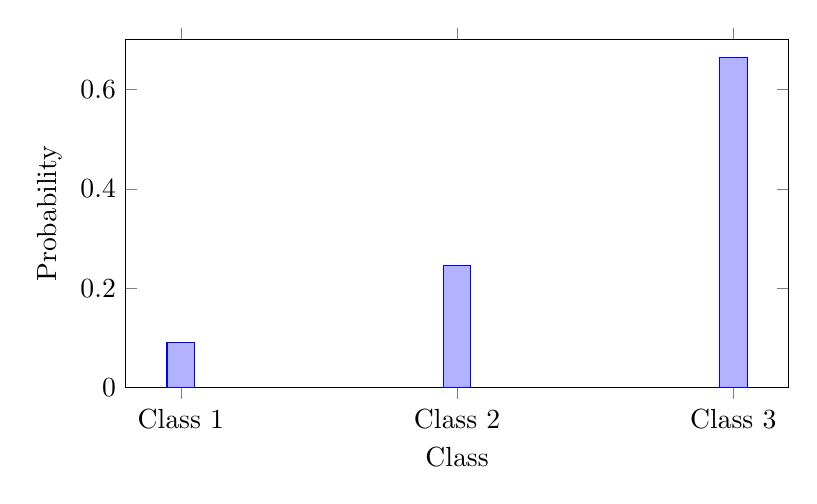
\begin{tikzpicture}
\begin{axis}[
    ylabel={Probability},
    xlabel={Class},
    ybar,
    ymin=0,
    ymax=0.7,
    width=10cm,
    height=6cm,
    xtick={1,2,3},
    xticklabels={Class 1, Class 2, Class 3}
]
\addplot coordinates {(1,0.090) (2,0.245) (3,0.665)};
\end{axis}
\end{tikzpicture}
\caption{Stable softmax computation for large inputs}
\label{fig:stable-softmax}
\end{figure}

\subsection{Other Numerical Issues}

\textbf{Catastrophic cancellation:} Loss of precision when subtracting nearly equal numbers.

\textbf{Accumulated rounding errors:} Small errors compound through many operations.

\textbf{Solutions:}
\begin{itemize}
    \item Use higher precision (64-bit floats)
    \item Algorithmic modifications (like log-sum-exp)
    \item Batch normalization
    \item Gradient clipping
\end{itemize}

% Chapter 4, Section 2: Gradient-Based Optimization

\section{Gradient-Based Optimization \difficultyInline{beginner}}
\label{sec:gradient-optimization}

Gradient-based optimization is the fundamental method for training deep learning models, using the mathematical concept of gradients to iteratively find optimal parameters that minimize loss functions through careful navigation of high-dimensional parameter spaces.

\subsection{Intuition: Finding the Bottom of a Hill}

Imagine you're hiking in foggy mountains and need to find the lowest point in a valley. You can't see far ahead, but you can feel the slope under your feet. The steepest downward direction tells you which way to walk to get lower. This is exactly what gradient descent does, where the mountain represents the loss function we want to minimize, your position represents the current parameter values, the slope represents the gradient (direction of steepest increase), and your steps represent parameter updates. Most deep learning algorithms involve optimization, which is the process of finding parameters that minimize or maximize an objective function, making gradient descent the cornerstone of neural network training.

\subsection{Gradient Descent}

For a function $f(\vect{\theta})$, \textbf{gradient descent} updates parameters as:

\begin{equation}
\vect{\theta}_{t+1} = \vect{\theta}_t - \alpha \nabla_{\vect{\theta}} f(\vect{\theta}_t)
\end{equation}

where $\alpha > 0$ is the \textbf{learning rate}.

\subsubsection{Example: Gradient Descent in 2D}

Consider minimizing $f(x, y) = x^2 + 2y^2$ starting from $(3, 3)$:

\begin{figure}[h]
\centering
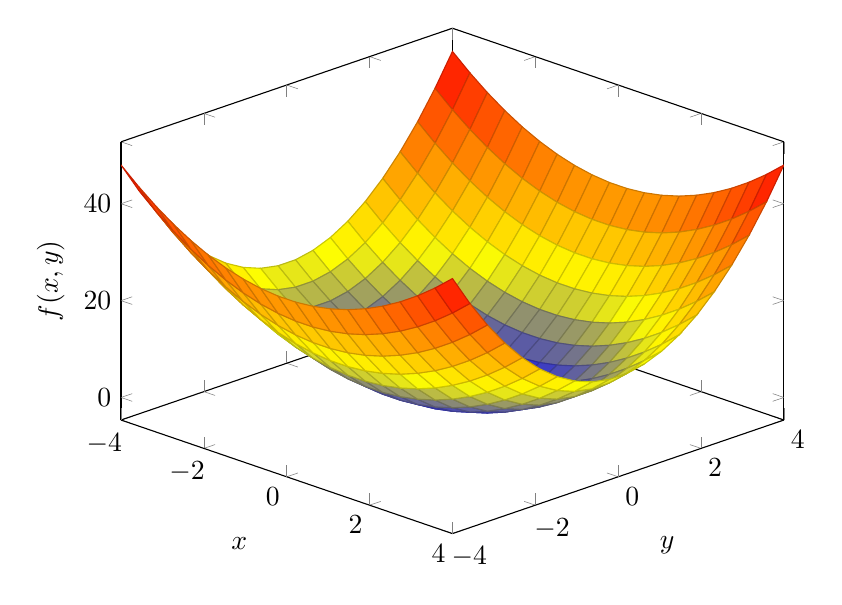
\begin{tikzpicture}
\begin{axis}[
    xlabel={$x$},
    ylabel={$y$},
    zlabel={$f(x,y)$},
    width=10cm,
    height=8cm,
    view={45}{30}
]
\addplot3[
    surf,
    domain=-4:4,
    domain y=-4:4,
    samples=20
] {x^2 + 2*y^2};
\end{axis}
\end{tikzpicture}
\caption{Contour plot of $f(x,y) = x^2 + 2y^2$ showing gradient descent path}
\label{fig:gradient-descent-2d}
\end{figure}

The gradient is $\nabla f = [2x, 4y]$. Starting from $(3, 3)$ with learning rate $\alpha = 0.1$:
\begin{align}
\nabla f(3, 3) &= [6, 12] \\
(x_1, y_1) &= (3, 3) - 0.1[6, 12] = (2.4, 1.8) \\
\nabla f(2.4, 1.8) &= [4.8, 7.2] \\
(x_2, y_2) &= (2.4, 1.8) - 0.1[4.8, 7.2] = (1.92, 1.08)
\end{align}

\subsection{Jacobian and Hessian Matrices}

The \textbf{Jacobian matrix} contains all first-order partial derivatives. For $\vect{f}: \mathbb{R}^n \to \mathbb{R}^m$:

\begin{equation}
\mat{J}_{ij} = \frac{\partial f_i}{\partial x_j}
\end{equation}

The \textbf{Hessian matrix} contains second-order derivatives:

\begin{equation}
\mat{H}_{ij} = \frac{\partial^2 f}{\partial x_i \partial x_j}
\end{equation}

The Hessian characterizes the local curvature of the function.

\subsection{Taylor Series Approximation}

Near point $\vect{x}_0$, we can approximate $f(\vect{x})$ using Taylor series:

\begin{equation}
f(\vect{x}) \approx f(\vect{x}_0) + (\vect{x} - \vect{x}_0)^\top \nabla f(\vect{x}_0) + \frac{1}{2}(\vect{x} - \vect{x}_0)^\top \mat{H}(\vect{x}_0) (\vect{x} - \vect{x}_0)
\end{equation}

This provides insight into optimization behavior.

\begin{example}[Taylor Series for $f(x) = e^x$ around $x_0 = 0$]
For the exponential function $f(x) = e^x$, we can compute the Taylor series expansion around $x_0 = 0$:

Since all derivatives of $e^x$ are $e^x$, and $e^0 = 1$, we have:
\begin{align}
f(0) &= 1 \\
f'(0) &= 1 \\
f''(0) &= 1 \\
f'''(0) &= 1 \\
&\vdots
\end{align}

The Taylor series expansion is:
\begin{equation}
e^x \approx 1 + x + \frac{x^2}{2!} + \frac{x^3}{3!} + \frac{x^4}{4!} + \cdots
\end{equation}

For small values of $x$, we can use the first few terms:
\begin{itemize}
    \item Linear approximation: $e^x \approx 1 + x$
    \item Quadratic approximation: $e^x \approx 1 + x + \frac{x^2}{2}$
    \item Cubic approximation: $e^x \approx 1 + x + \frac{x^2}{2} + \frac{x^3}{6}$
\end{itemize}

For example, $e^{0.1} \approx 1 + 0.1 + \frac{0.01}{2} = 1.105$, which is very close to the true value of approximately $1.1052$.
\end{example}

\subsection{Critical Points}

Critical points are locations where the gradient is zero, representing different types of terrain features in the optimization landscape. A local minimum is like the bottom of a bowl where you can't go lower in any direction, a local maximum is like the top of a hill where you can't go higher in any direction, and a saddle point is like a mountain pass where you can go down in some directions and up in others. At a critical point, $\nabla f(\vect{x}) = \boldsymbol{0}$, and the Hessian matrix determines the nature of the critical point: a local minimum occurs when the Hessian is positive definite, a local maximum occurs when the Hessian is negative definite, and a saddle point occurs when the Hessian has both positive and negative eigenvalues.

\begin{figure}[h]
\centering
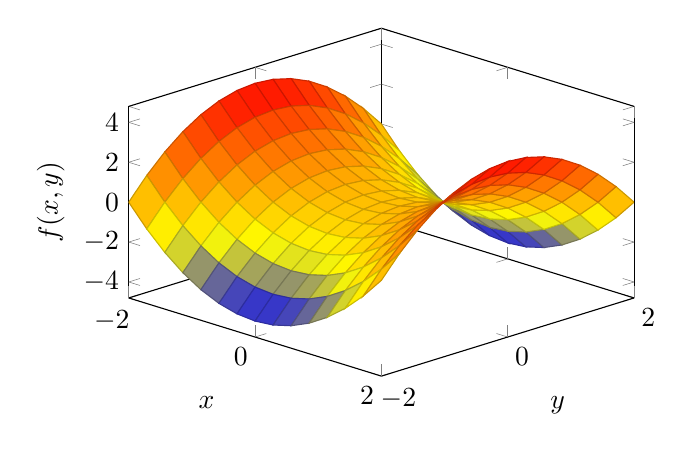
\begin{tikzpicture}
\begin{axis}[
    xlabel={$x$},
    ylabel={$y$},
    zlabel={$f(x,y)$},
    width=8cm,
    height=6cm,
    view={45}{30}
]
\addplot3[
    surf,
    domain=-2:2,
    domain y=-2:2,
    samples=15
] {x^2 - y^2};
\end{axis}
\end{tikzpicture}
\caption{Example of a saddle point: $f(x,y) = x^2 - y^2$}
\label{fig:saddle-point}
\end{figure}

Deep learning often encounters saddle points rather than local minima in high dimensions.

\subsection{Directional Derivatives}

The directional derivative in direction $\vect{u}$ (with $\|\vect{u}\| = 1$) is:

\begin{equation}
\frac{\partial}{\partial \alpha} f(\vect{x} + \alpha \vect{u}) \bigg|_{\alpha=0} = \vect{u}^\top \nabla f(\vect{x})
\end{equation}

To minimize $f$, we move in the direction $\vect{u} = -\frac{\nabla f(\vect{x})}{\|\nabla f(\vect{x})\|}$.

% Chapter 4, Section 3: Constrained Optimization

\section{Constrained Optimization \difficultyInline{beginner}}
\label{sec:constrained-optimization}

Constrained optimization extends traditional optimization by incorporating additional requirements or limitations that must be satisfied while finding optimal solutions, providing essential tools for implementing regularization, fairness constraints, and other practical considerations in deep learning applications.

\subsection{Intuition: Optimization with Rules}

Imagine you're trying to find the best location for a new store, but you have constraints such as being within 10 km of the city centre, having parking for at least 50 cars, and a budget that cannot exceed \$1 million. You can't just pick any location - you must follow these rules while still optimizing your objective like maximizing customer traffic. In deep learning, we often have similar constraints including weight constraints to keep weights small and prevent overfitting, probability constraints where outputs must sum to 1 like in softmax functions, and fairness constraints where the model must treat different groups equally. Many problems require optimizing a function subject to constraints, making constrained optimization an essential tool for practical machine learning applications.

\subsection{Lagrange Multipliers}

For equality constraint $g(\vect{x}) = 0$, the \textbf{Lagrangian} is:

\begin{equation}
\mathcal{L}(\vect{x}, \lambda) = f(\vect{x}) + \lambda g(\vect{x})
\end{equation}

At the optimum, both:
\begin{equation}
\nabla_{\vect{x}} \mathcal{L} = \boldsymbol{0} \quad \text{and} \quad \frac{\partial \mathcal{L}}{\partial \lambda} = 0
\end{equation}

\begin{remark}
Lagrange multipliers are crucial in deep learning for implementing regularization techniques like weight decay and dropout, where we optimize the loss function subject to constraints on parameter norms or activation patterns. They also enable the development of constrained optimization algorithms for training neural networks with fairness constraints, ensuring models treat different demographic groups equally while maintaining high performance.
\end{remark}

\subsection{Inequality Constraints}

For inequality constraint $g(\vect{x}) \leq 0$, we use the \textbf{Karush-Kuhn-Tucker (KKT)} conditions:

\begin{align}
\nabla_{\vect{x}} \mathcal{L} &= \boldsymbol{0} \\
\lambda &\geq 0 \\
\lambda g(\vect{x}) &= 0 \quad \text{(complementary slackness)} \\
g(\vect{x}) &\leq 0
\end{align}

\begin{remark}
KKT conditions are essential in deep learning for handling inequality constraints such as bounding neural network weights to prevent exploding gradients, ensuring activation functions stay within valid ranges, and implementing robust optimization with adversarial training where perturbations must remain within specified bounds. They also enable the development of constrained optimization algorithms for training neural networks with fairness constraints, ensuring models treat different demographic groups equally while maintaining high performance.
\end{remark}

\subsection{Projected Gradient Descent}

For constraints defining a set $\mathcal{C}$, \textbf{projected gradient descent} applies:

\begin{equation}
\vect{x}_{t+1} = \text{Proj}_{\mathcal{C}}\left(\vect{x}_t - \alpha \nabla f(\vect{x}_t)\right)
\end{equation}

where $\text{Proj}_{\mathcal{C}}$ projects onto the feasible set.

The mathematical operation works as follows: first, we compute the standard gradient descent step $\vect{x}_t - \alpha \nabla f(\vect{x}_t)$, which may move us outside the feasible set $\mathcal{C}$. Then, the projection operator $\text{Proj}_{\mathcal{C}}$ finds the closest point in $\mathcal{C}$ to this intermediate result, ensuring that $\vect{x}_{t+1} \in \mathcal{C}$. The projection is defined as:
\begin{equation}
\text{Proj}_{\mathcal{C}}(\vect{y}) = \arg\min_{\vect{x} \in \mathcal{C}} \|\vect{x} - \vect{y}\|_2
\end{equation}

This ensures that each update step remains within the constraint set while still moving in the direction that reduces the objective function.

\begin{remark}
Projected gradient descent is essential in deep learning for maintaining constraints during training, such as keeping neural network weights within specified bounds to prevent exploding gradients, ensuring probability outputs sum to 1 in softmax layers, and implementing robust optimization with adversarial training where perturbations must stay within $\ell_\infty$ balls around input examples.
\end{remark}

\subsection{Applications in Deep Learning}

Constrained optimization appears in several important applications in deep learning, including weight constraints such as unit norm constraints that help prevent overfitting and improve generalization, projection to valid probability distributions that ensures model outputs are mathematically valid, adversarial training with bounded perturbations that creates robust models by training against carefully crafted adversarial examples, and fairness constraints that ensure models treat different groups equally and avoid discriminatory behavior.

% Chapter 4, Section 4: Numerical Stability and Conditioning

\section{Numerical Stability and Conditioning \difficultyInline{beginner}}
\label{sec:numerical-stability}

\subsection{Intuition: The Butterfly Effect in Computation}

Imagine a house of cards. A tiny breeze can cause the entire structure to collapse. In numerical computation, we have a similar problem: small errors can grow into large ones.

This is especially problematic in deep learning because:
\begin{itemize}
    \item \textbf{Deep networks} have many layers - errors compound
    \item \textbf{Matrix operations} can amplify small errors
    \item \textbf{Gradient computation} requires precise derivatives
\end{itemize}

The \textbf{condition number} tells us how "sensitive" a computation is to small changes. A high condition number means small input errors become large output errors.

\subsection{Condition Number}

The \textbf{condition number} of matrix $\mat{A}$ is:

\begin{equation}
\kappa(\mat{A}) = \|\mat{A}\| \|\mat{A}^{-1}\|
\end{equation}

For symmetric matrices with eigenvalues $\lambda_i$:

\begin{equation}
\kappa(\mat{A}) = \frac{\max_i |\lambda_i|}{\min_i |\lambda_i|}
\end{equation}

High condition numbers indicate numerical instability: small changes in input lead to large changes in output.

\subsubsection{Example: Well-Conditioned vs Ill-Conditioned Matrices}

Consider two matrices:
\begin{align}
\mat{A}_1 &= \begin{bmatrix} 2 & 0 \\ 0 & 2 \end{bmatrix} \quad \text{(well-conditioned)} \\
\mat{A}_2 &= \begin{bmatrix} 1 & 0.99 \\ 0.99 & 1 \end{bmatrix} \quad \text{(ill-conditioned)}
\end{align}

\begin{figure}[h]
\centering
\begin{tikzpicture}
\begin{axis}[
    xlabel={Input Error},
    ylabel={Output Error},
    width=10cm,
    height=6cm,
    legend pos=north west
]
\addplot[bookpurple, thick] {x};
\addplot[bookred, thick] {10*x};
\legend{Well-conditioned, Ill-conditioned}
\end{axis}
\end{tikzpicture}
\caption{Error amplification for well-conditioned vs ill-conditioned matrices}
\label{fig:condition-number}
\end{figure}

\subsection{Ill-Conditioned Matrices}

In deep learning, ill-conditioned Hessians can make optimization difficult. This motivates techniques like:
\begin{itemize}
    \item Batch normalization
    \item Careful weight initialization
    \item Adaptive learning rate methods
    \item Preconditioning
\end{itemize}

\subsection{Gradient Checking}

To verify gradient computations, we use \textbf{finite differences}:

\begin{equation}
\frac{\partial f}{\partial \theta_i} \approx \frac{f(\theta_i + \epsilon) - f(\theta_i - \epsilon)}{2\epsilon}
\end{equation}

This is computationally expensive but useful for debugging.

\subsection{Numerical Precision Trade-offs}

\textbf{Mixed precision training:}
\begin{itemize}
    \item Store weights in FP32
    \item Compute activations/gradients in FP16
    \item Use loss scaling to prevent underflow
    \item 2-3x speedup with minimal accuracy loss
\end{itemize}

\subsection{Practical Tips}

\begin{itemize}
    \item Monitor gradient norms during training
    \item Use gradient clipping for RNNs
    \item Prefer numerically stable implementations (log-space computations)
    \item Be aware of precision limits in very deep networks
\end{itemize}


% Chapter summary and exercises
% Key Takeaways for Chapter 4

\section*{Key Takeaways}
\addcontentsline{toc}{section}{Key Takeaways}

\begin{keytakeaways}
\begin{itemize}[leftmargin=2em]
    \item \textbf{Numerical precision} matters: Finite precision arithmetic can cause overflow, underflow, and instability in deep learning computations.
    \item \textbf{Gradient-based optimisation} relies on Jacobian and Hessian matrices to navigate loss landscapes and find optimal parameters.
    \item \textbf{Constrained optimisation} uses Lagrange multipliers and KKT conditions to solve problems with constraints.
    \item \textbf{Numerical stability} is assessed via condition numbers; ill-conditioned problems require careful handling.
    \item \textbf{Practical techniques} like log-sum-exp tricks and gradient checking ensure robust implementations.
\end{itemize}
\end{keytakeaways}



% Exercises (Hands-On Exercises) for Chapter 4: Numerical Computation

\section*{Exercises}
\addcontentsline{toc}{section}{Exercises}

\subsection*{Easy}

\begin{exercisebox}[easy]
\begin{problem}[Floating-Point Basics]
\label{prob:float-basics}
Consider a hypothetical 4-bit floating-point system with 1 sign bit, 2 exponent bits, and 1 mantissa bit. What is the smallest positive number that can be represented? What is the largest number?
\end{problem}
\begin{hintbox}
Use the IEEE 754 format: $(-1)^s \times 2^{e-b} \times (1 + m)$ where $s$ is the sign bit, $e$ is the exponent, $b$ is the bias, and $m$ is the mantissa.
\end{hintbox}
\end{exercisebox}


\begin{exercisebox}[easy]
\begin{problem}[Softmax Stability]
\label{prob:softmax-stability}
Compute the softmax of $\vect{x} = [1000, 1001, 1002]$ using both the naive approach and the numerically stable approach. Show your work step by step.
\end{problem}
\begin{hintbox}
Use the identity $\text{softmax}(\vect{x}) = \text{softmax}(\vect{x} - c)$ where $c = \max_i x_i$.
\end{hintbox}
\end{exercisebox}


\begin{exercisebox}[easy]
\begin{problem}[Gradient Computation]
\label{prob:gradient-computation}
Compute the gradient of $f(x, y) = x^2 + 3xy + y^2$ at the point $(2, 1)$.
\end{problem}
\begin{hintbox}
The gradient is $\nabla f = \left[\frac{\partial f}{\partial x}, \frac{\partial f}{\partial y}\right]$.
\end{hintbox}
\end{exercisebox}


\begin{exercisebox}[easy]
\begin{problem}[Condition Number]
\label{prob:condition-number}
Calculate the condition number of the matrix $\mat{A} = \begin{bmatrix} 1 & 0.5 \\ 0.5 & 1 \end{bmatrix}$.
\end{problem}
\begin{hintbox}
For a 2×2 matrix, $\kappa(\mat{A}) = \frac{\lambda_{\max}}{\lambda_{\min}}$ where $\lambda_{\max}$ and $\lambda_{\min}$ are the eigenvalues.
\end{hintbox}
\end{exercisebox}


\begin{exercisebox}[easy]
\begin{problem}[Numerical Differentiation]
\label{prob:numerical-diff}
Implement the forward, backward, and central difference formulas for computing the derivative of $f(x) = \sin(x)$ at $x = \pi/4$. Compare the accuracy with the analytical derivative.
\end{problem}
\begin{hintbox}
Use $f'(x) \approx \frac{f(x+h) - f(x)}{h}$ for forward difference and similar formulas for other methods.
\end{hintbox}
\end{exercisebox}


\begin{exercisebox}[easy]
\begin{problem}[Machine Epsilon]
\label{prob:machine-epsilon}
Write a program to find the machine epsilon of your system. What is the smallest number $\epsilon$ such that $1 + \epsilon \neq 1$ in floating-point arithmetic?
\end{problem}
\begin{hintbox}
Start with $\epsilon = 1$ and repeatedly divide by 2 until $1 + \epsilon = 1$.
\end{hintbox}
\end{exercisebox}


\begin{exercisebox}[easy]
\begin{problem}[Numerical Integration]
\label{prob:numerical-integration}
Compare the trapezoidal rule and Simpson's rule for approximating $\int_0^1 e^{-x^2} dx$. Use $n = 4, 8, 16$ subintervals.
\end{problem}
\begin{hintbox}
Trapezoidal rule: $\int_a^b f(x)dx \approx \frac{h}{2}[f(a) + 2\sum_{i=1}^{n-1}f(x_i) + f(b)]$.
\end{hintbox}
\end{exercisebox}


\begin{exercisebox}[easy]
\begin{problem}[Matrix Conditioning]
\label{prob:matrix-conditioning}
Given the matrix $\mat{A} = \begin{bmatrix} 1 & 1 \\ 1 & 1.0001 \end{bmatrix}$, compute its condition number and solve $\mat{A}\vect{x} = \vect{b}$ where $\vect{b} = [2, 2.0001]^T$.
\end{problem}
\begin{hintbox}
A small change in $\vect{b}$ can cause a large change in the solution when the condition number is large.
\end{hintbox}
\end{exercisebox}


\subsection*{Medium}

\begin{exercisebox}[medium]
\begin{problem}[Log-Sum-Exp Trick]
\label{prob:log-sum-exp}
Derive the log-sum-exp trick: $\log\left(\sum_{i=1}^n \exp(x_i)\right) = c + \log\left(\sum_{i=1}^n \exp(x_i - c)\right)$ where $c = \max_i x_i$.
\end{problem}
\begin{hintbox}
Start by factoring out $\exp(c)$ from the sum.
\end{hintbox}
\end{exercisebox}


\begin{exercisebox}[medium]
\begin{problem}[Lagrange Multipliers]
\label{prob:lagrange-multipliers}
Find the maximum value of $f(x, y) = xy$ subject to the constraint $x^2 + y^2 = 1$ using Lagrange multipliers.
\end{problem}
\begin{hintbox}
Set up the Lagrangian $\mathcal{L}(x, y, \lambda) = xy + \lambda(1 - x^2 - y^2)$ and solve the system of equations.
\end{hintbox}
\end{exercisebox}


\begin{exercisebox}[medium]
\begin{problem}[Gradient Descent Convergence]
\label{prob:gradient-convergence}
For the function $f(x, y) = x^2 + 100y^2$, implement gradient descent with different learning rates. Show that the convergence rate depends on the condition number.
\end{problem}
\begin{hintbox}
The condition number of the Hessian matrix determines the convergence rate.
\end{hintbox}
\end{exercisebox}


\begin{exercisebox}[medium]
\begin{problem}[Newton's Method]
\label{prob:newton-method}
Use Newton's method to find the root of $f(x) = x^3 - 2x - 5$ starting from $x_0 = 2$. Compare with the bisection method.
\end{problem}
\begin{hintbox}
Newton's method: $x_{n+1} = x_n - \frac{f(x_n)}{f'(x_n)}$.
\end{hintbox}
\end{exercisebox}


\begin{exercisebox}[medium]
\begin{problem}[Eigenvalue Computation]
\label{prob:eigenvalue-computation}
For the matrix $\mat{A} = \begin{bmatrix} 3 & 1 \\ 1 & 3 \end{bmatrix}$, compute the eigenvalues and eigenvectors using the characteristic equation and verify with numerical methods.
\end{problem}
\begin{hintbox}
Solve $\det(\mat{A} - \lambda\mat{I}) = 0$ for eigenvalues.
\end{hintbox}
\end{exercisebox}


\subsection*{Hard}

\begin{exercisebox}[hard]
\begin{problem}[Numerical Stability of Matrix Inversion]
\label{prob:matrix-inversion-stability}
Consider the matrix $\mat{A} = \begin{bmatrix} 1 & 1 \\ 1 & 1 + \epsilon \end{bmatrix}$ where $\epsilon$ is small. Show that the condition number grows as $\epsilon \to 0$. Implement a numerical experiment to demonstrate this and show how the error in $\mat{A}^{-1}$ grows.
\end{problem}
\begin{hintbox}
Use the formula $\kappa(\mat{A}) = \frac{\lambda_{\max}}{\lambda_{\min}}$ and compute the eigenvalues analytically.
\end{hintbox}
\end{exercisebox}


\begin{exercisebox}[hard]
\begin{problem}[KKT Conditions Application]
\label{prob:kkt-conditions}
Consider the optimisation problem:
\begin{align}
\min_{x, y} \quad & x^2 + y^2 \\
\text{subject to} \quad & x + y \geq 1 \\
& x \geq 0, y \geq 0
\end{align}
Find the optimal solution using the KKT conditions and verify that all conditions are satisfied.
\end{problem}
\begin{hintbox}
Set up the Lagrangian with multiple constraints and check the complementary slackness conditions.
\end{hintbox}
\end{exercisebox}


